\chapter{Results and Discussion}\label{chapter:results}
This chapter includes presentation and analysis of the results obtained in this thesis. Section \ref{section:parameter settings} presents results from testing different parameter settings for the genetic algorithm, and briefly discusses each results. Section \ref{section:results} presents the main results obtained when running the different population distributed genetic algorithms. Section \ref{section:discussion} contains a discussion and comparison of the results obtained in section \ref{section:results}.


\section{Parameter settings}\label{section:parameter settings}
Parameter settings are crucial for obtaining good results with the genetic algorithm. In order to find the right settings, simulations were run to find the best adult selection method, parent selection method, crossover method, crossover rate and mutation rate for the given problem. Even though it would take much shorter time and less effort to test these settings on a toy problem such as One Max, the decision was made to test them on the real problem. The reason behind this decision is that different settings might work better on different problems and the nature of the wind farm layout optimization problem is unique because of the importance of the wind turbine positions relative to each other. It is important to note that even though effort was made to find good settings for the genetic algorithm,  it is impossible to obtain the optimal ones. Just imagine trying the test every single value for the continuous parameter crossover rate against every possible value of each of the other settings, just that would be impossible! Therefore, the values that are tested for each parameter setting is largely tested against values that are based on the authors previous experience with genetic algorithm and values close to those.\\

\begin{table}
\centering
\caption{Values kept fixed while one by one was changed in order to find the best settings for the wind farm layout optimization problem.}
\label{table:fixed settings}
\begin{tabular}{l|l}
\textbf{Parameter} & \textbf{Value} \\ 
\hline 
Wind scenario & 00.xml \\ 
Evaluator & KusiakLayoutEvaluator \\ 
Population size & 100 \\  
Generations & 100 \\ 
Elitism & true \\  
Flip mutation rate & 0.01 \\ 
Inversion mutation rate & 0.0 \\ 
Interchange mutation rate & 0.0 \\ 
Parent selection & Tournament selection \\ 
Tournament size & 5 \\ 
Epsilon & 0.0 \\  
Crossover method & Uniform crossover \\ 
Crossover rate & 0.9 \\ 
\end{tabular} 
\end{table}

\noindent For each simulation one of the parameters were tested while the others were kept fixed as shown in table \ref{table:fixed settings}. As can be seen in this table, other settings such as wind scenario, population size, number of generations, whether elitism should be used and mutation rate for interchange mutation and inversion mutation could also be tested, but since evaluation of each farm takes a lot of time, even on an 8 core computer running in parallel, simulations are not run to set these values. These settings are set using the authors previous experience and educated guessing. Testing different parameters on a single wind scenario might lead to values that are tailored for the given scenario and that are not as well suited for some of the others. However, there is no time to test each value for every single wind scenario, and this should not make that much of a difference. Population size is a value that influence the performance of the genetic algorithm largely. Greater population size often leads to better performance since more solutions increase the probability of finding the global optimal solution. The population size was set to 100 for two reasons. First of all, a population size of 100 is large enough so that many different solutions are explored. Second when the population size is kept at 100, the adult selection method ''Overproduction'' will produce twice as many children, so that 200 individuals has to be evaluated for each generation something that will double the evaluation time, the step that already is the bottleneck of the algorithm. The number of generations was kept at 100 for each run, evaluating each population for 100 generations takes time and it the main reason why the algorithm were not run for more generations, however, as can be seen on the graphs in the sections below the fitness looks like it is starting to flat out after a 100 generations indicating that a 100 generations are sufficient for the purpose of setting the parameter values. Elitism was set to true for every run without testing, meaning that the best individual of each generation will survive. This decision is based on the authors previous experience with genetic algorithm where experiments has shown that elitism leads to better results because the best individual is not lost due to coincidences. Different mutation methods were implemented for the genetic algorithm, but only the flip mutation rate was tested to find the best value. Usually, flip mutation is the only mutation method used with genetic algorithms and it is therefore also used as the main for of mutation in this thesis. Inversion mutation and interchange mutation are implemented, but they will only happen seldom to introduce more randomness to the algorithm. In the main simulations, they will be assigned extremely low probabilities so that their occurrence is so rare that they will introduce too much randomness, but hopefully make occasional ''jumps'' to different solutions spaces so that the algorithm do not get completely stuck in a local optimal solution. 


\subsection{Adult Selection}
Figure \ref{figure:adult selection methods} shows the results of running the genetic algorithm with the different adult selection methods. Figure \ref{figure:full generational replacement}, \ref{figure:generational mixing}, and \ref{figure:overproduction} shows the results for full generational replacement, generational mixing and overproduction respectively. 

As can be seen in the figures, full generational replacement ends up with lower fitness than both generational mixing and overproduction, and overproduction ends up with best fitness. These results are as expected. Note that generational mixing could never do worse than full generational replacement. If the results of reproduction leads to a population of individuals with strictly better fitness, generational mixing will replace the entire previous generation with the new one, as full generational replacement. However, if the new generation produces individuals with worse fitness than some of the individuals in the previous generation these old individuals will be kept instead, making sure that the new population has equal or better fitness than the previous one. Overproduction does not provide the same ''newer worst'' \textcolor{red}{Check word!} guarantee, however, as shown in figure \ref{figure:overproduction} it still outperforms generational mixing. Even though overproduction wipes out the entire previous population, it generates twice as many children at the reproduction step so its probability of getting it right is doubled. 


\begin{figure}[h!]
    \centering
    \begin{subfigure}[b]{0.31\textwidth}
        \includegraphics[width=\textwidth]{images/plots/"adult selection"/"full generational replacement"}
        \caption{}
        \hfill
        \label{plot:full generational replacement}
    \end{subfigure}
    ~
    \begin{subfigure}[b]{0.31\textwidth}
        \includegraphics[width=\textwidth]{images/plots/"adult selection"/"generational mixing"}
        \caption{}
        \hfill
        \label{plot:generational mixing}
    \end{subfigure}
    ~
    \begin{subfigure}[b]{0.31\textwidth}
        \includegraphics[width=\textwidth]{images/plots/"adult selection"/"overproduction"}
        \caption{}
        \hfill
        \label{plot:overproduction}
    \end{subfigure}
    \caption{Adult selection methods: (a) Full generational replacement, (b) generational mixing and (c) overproduction averaged over 10 runs.}
    \label{plot:adult selection methods}
\end{figure}


\subsection{Parent Selection}
Figure \ref{plot:parent selection} shows the results for running the genetic algorithm with parent selection method roulette wheel \ref{plot:roulette wheel}, and tournament selection \ref{plot:tournament size 5} - \ref{plot:tournament size 25}. Tournament selection is run with five different values for the variable \textit{tournament size}. Clearly, tournament selection beats roulette wheel by far. The problem with roulette wheel is that it assigns each individual a probability of being selected proportional to its fitness, since there is not a large difference in fitness for the different individuals the selection becomes almost random. \\


\noindent As can be seen in the figure, the fitness gets better as the variable \textit{tournament size} increases. However, a larger tournament size than 25 is not tested. The reason for this is that 25 is already a very large tournament size. With 25 \% of the individuals competing in every tournament the population will not have much time to explore different solutions because the best individuals will soon take over the entire population. As can be seen in the figure, a tournament size of 25 is only slightly better than a tournament size of 20, and therefore 20 is chosen as the final tournament size to slow down the take-over time. \\


\noindent As mentioned before, \textit{epsilon} is the probability that the selected individual is selected from a random position in the adult pool instead of by tournament selection. Figure \ref{plot:epsilon} shows the result for testing the values 5 \%, 10 \%, and 15 \%. As can be seen in the figure, varying epsilon does not have much impact on the fitness.\\


\begin{figure}[h!]
    \centering
    \begin{subfigure}[b]{0.31\textwidth}
        \includegraphics[width=\textwidth]{images/plots/"parent selection"/"roulette wheel"}
        \caption{}
        \hfill
        \label{plot:roulette wheel}
    \end{subfigure}
    ~
    \begin{subfigure}[b]{0.31\textwidth}
        \includegraphics[width=\textwidth]{images/plots/"parent selection"/"tournament size 5"}
        \caption{}
        \hfill
        \label{plot:tournament size 5}
    \end{subfigure}
    ~
       \begin{subfigure}[b]{0.31\textwidth}
        \includegraphics[width=\textwidth]{images/plots/"parent selection"/"tournament size 10"}
        \caption{}
        \hfill
        \label{plot:tournament size 10}
    \end{subfigure}
    ~
       \begin{subfigure}[b]{0.31\textwidth}
        \includegraphics[width=\textwidth]{images/plots/"parent selection"/"tournament size 15"}
        \caption{}
        \hfill
        \label{plot:tournament size 15}
    \end{subfigure}
    ~
       \begin{subfigure}[b]{0.31\textwidth}
        \includegraphics[width=\textwidth]{images/plots/"parent selection"/"tournament size 20"}
        \caption{}
        \hfill
        \label{plot:tournament size 20}
    \end{subfigure}
    ~
    \begin{subfigure}[b]{0.31\textwidth}
        \includegraphics[width=\textwidth]{images/plots/"parent selection"/"tournament size 25"}
        \caption{}
        \hfill
        \label{plot:tournament size 25}
    \end{subfigure}
    \caption{Parent selection methods: (a) Roulette wheel, (b) Tournament selection averaged over 10 runs, tournament size 5 (c) tournament selection, tournament size 10, (d) tournament selection, tournament size 15, (e) tournament selection, tournaments size 20, and (f) tournament selection, tournament size 25.}
    \label{plot:parent selection}
\end{figure}


\begin{figure}[h!]
    \centering
    \begin{subfigure}[b]{0.31\textwidth}
        \includegraphics[width=\textwidth]{images/plots/epsilon/"tournament size 20"/"epsilon 0,05"}
        \caption{}
        \hfill
        \label{plot:epsilon 0.05}
    \end{subfigure}
    ~
    \begin{subfigure}[b]{0.31\textwidth}
        \includegraphics[width=\textwidth]{images/plots/epsilon/"tournament size 20"/"epsilon 0,10"}
        \caption{}
        \hfill
        \label{plot:epsilon 0.10}
    \end{subfigure}
    ~
    \begin{subfigure}[b]{0.31\textwidth}
        \includegraphics[width=\textwidth]{images/plots/epsilon/"tournament size 20"/"epsilon 0,15"}
        \caption{}
        \hfill
        \label{plot:epsilon 0.15}
    \end{subfigure}
    \caption{Different epsilon values averaged 10 runs when tournament size was kept at 20: (a) Epsilon 0.05, (b) epsilon 0.10 and (c) epsilon 0.15.}
    \label{plot:epsilon}
\end{figure}


\subsection{Crossover Methods}
Figure \ref{figure:crossover methods} displays the results from running the genetic algorithm with single point crossover, two point crossover and uniform crossover showed in sub figures \ref{figure:single point crossover}, \ref{figure:two point crossover} and \ref{figure:uniform crossover} respectively. As can be seen in the figure, there is no crossover method that stands out, but end up with similar fitness. Single point crossover ends up with an averaged best fitness of \textcolor{red}{averaged best fitness}, two point crossover ends up with an averaged fitness of \textcolor{red}{averaged best fitness} and uniform crossover ends up with an averaged fitness of \textcolor{red}{averaged best fitness}. Intuitively, one would expect uniform crossover to perform worse than the others because it mixes up the relative positions between the wind turbines more than single- and two point crossover, however it actually obtains slightly better fitness. Even though it obtains slightly better fitness this could be a coincidence since the different is so small, and the simulations are only averaged over ten runs. \textcolor{red}{Explanation behind the results, talk to Keith. Stupid paragraph change everything!}


\begin{figure}[h!]
    \centering
    \begin{subfigure}[b]{0.31\textwidth}
        \includegraphics[width=\textwidth]{images/plots/"crossover method"/"single point crossover"}
        \caption{}
        \hfill
        \label{plot:single point crossover}
    \end{subfigure}
    ~
    \begin{subfigure}[b]{0.31\textwidth}
        \includegraphics[width=\textwidth]{images/plots/"crossover method"/"two point crossover"}
        \caption{}
        \hfill
        \label{plot:two point crossover}
    \end{subfigure}
    ~
    \begin{subfigure}[b]{0.31\textwidth}
        \includegraphics[width=\textwidth]{images/plots/"crossover method"/"uniform crossover"}
        \caption{}
        \hfill
        \label{plot:uniform crossover}
    \end{subfigure}
    \caption{Crossover methods averaged over 10 runs: (a) Single point crossover, (b) two point crossover and (c) uniform crossover.}
    \label{plot:crossover methods}
\end{figure}


\subsection{Crossover Rate}


\begin{figure}[h!]
    \centering
    \begin{subfigure}[b]{0.31\textwidth}
        \includegraphics[width=\textwidth]{images/plots/"crossover rate"/"crossover rate 0,0"}
        \caption{}
        \hfill
        \label{plot:crossover rate 0.0}
    \end{subfigure}
    ~
    \begin{subfigure}[b]{0.31\textwidth}
        \includegraphics[width=\textwidth]{images/plots/"crossover rate"/"crossover rate 0,2"}
        \caption{}
        \hfill
        \label{plot:two point crossover}
    \end{subfigure}
    ~
       \begin{subfigure}[b]{0.31\textwidth}
        \includegraphics[width=\textwidth]{images/plots/"crossover rate"/"crossover rate 0,4"}
        \caption{}
        \hfill
        \label{plot:two point crossover}
    \end{subfigure}
    ~
       \begin{subfigure}[b]{0.31\textwidth}
        \includegraphics[width=\textwidth]{images/plots/"crossover rate"/"crossover rate 0,6"}
        \caption{}
        \hfill
        \label{plot:two point crossover}
    \end{subfigure}
    ~
       \begin{subfigure}[b]{0.31\textwidth}
        \includegraphics[width=\textwidth]{images/plots/"crossover rate"/"crossover rate 0,8"}
        \caption{}
        \hfill
        \label{plot:two point crossover}
    \end{subfigure}
    ~
    \begin{subfigure}[b]{0.31\textwidth}
        \includegraphics[width=\textwidth]{images/plots/"crossover rate"/"crossover rate 1,0"}
        \caption{}
        \hfill
        \label{plot:uniform crossover}
    \end{subfigure}
    \caption{Crossover rates: (a) Crossover rate 0.0, (b) crossover rate 0.2, (c) crossover rate 0.4, (d) crossover rate 0.6, (e) crossover rate 0.8, and (f) crossover rate 1.0.}
    \label{plot:crossover methods}
\end{figure}


\subsection{Mutation Rate}
In figure \ref{plot:mutation rate} the effect of varying the mutation rate can be seen. As the figure shows, if the mutation rate is very low (0.0001), the population is clearly not able to find a good solution. Mutation means adding or removing a turbine. As the figure shows, a mutation rate that is too low (0.0001) might not be able to add or remove enough turbines and therefore the population ends up at a local minima. On the other side, when the mutation rate gets too high (0.01) the population might be able to find the global minima, but, since mutation is performed too frequently, it is not able to stay there. As the figure shows, mutation rate largely impacts the fitness, and a mutation rate of 0.001 clearly gives the best results.


\begin{figure}[h!]
    \centering
      \begin{subfigure}[b]{0.31\textwidth}
        \includegraphics[width=\textwidth]{images/plots/"mutation rate"/"mutation rate 0,0001"}
        \caption{}
        \hfill
        \label{plot:mutation rate 0.0001}
    \end{subfigure}
    ~
      \begin{subfigure}[b]{0.31\textwidth}
        \includegraphics[width=\textwidth]{images/plots/"mutation rate"/"mutation rate 0,0005"}
        \caption{}
        \hfill
        \label{plot:mutation rate 0.0005}
    \end{subfigure}
    ~
    \begin{subfigure}[b]{0.31\textwidth}
        \includegraphics[width=\textwidth]{images/plots/"mutation rate"/"mutation rate 0,001"}
        \caption{}
        \hfill
        \label{plot:mutation rate 0.001}
    \end{subfigure}
    ~
    \begin{subfigure}[b]{0.31\textwidth}
        \includegraphics[width=\textwidth]{images/plots/"mutation rate"/"mutation rate 0,005"}
        \caption{}
        \hfill
        \label{plot:mutation rate 0.005}
    \end{subfigure}
    ~
    \begin{subfigure}[b]{0.31\textwidth}
        \includegraphics[width=\textwidth]{images/plots/"mutation rate"/"mutation rate 0,01"}
        \caption{}
        \hfill
        \label{plot:mutation rate 0.01}
    \end{subfigure}
    \caption{Mutation rates: (a) Mutation rate 0.0001, (b) mutation rate 0.0005 and (c) mutation rate 0.001, (d) mutation rate 0.005 and (e) mutation rate 0.01s.}
    \label{plot:mutation rate}
\end{figure}


\section{Results}\label{section:results}


\subsection{Parameter Settings}


\noindent In table \ref{table:final parameter settings master slave model}, the parameter values used when running the master slave model is shown. The crossover method, crossover rate, mutation rate, adult selection mechanism, parent selection mechanism and parent selection parameters are those that proved to work best for the wind farm layout optimization problem as shown in the previous section. The population size was set to 100 and the number of generations to 200. A population size of 100 is quite small, but since overproduction is the selected adult selection method a population size of 100 leads to evaluation of 200 individuals each generation. Since evaluation is the bottle neck, by far, for wind farm layout optimization a larger population size would not be possible to evaluate for 200 generations within the time limits of this thesis. A possibility could be to pick a larger population size and a smaller number of generations, but since the objective of this thesis is to explore population distributed genetic algorithms a large number of generations is crucial since population distributed genetic algorithms need more time to find good solutions because they need time to explore different parts of the search space. \\


\begin{table}[h!]
\centering
\caption{Parameter values used for the master slave model.}
\label{table:final parameter settings master slave model}
\begin{tabular}{l|l}
\textbf{Parameter} & \textbf{Value} \\ 
\hline 
Population size & 100 \\  
Generations & 200 \\ 
Crossover method & Single point crossover \\ 
Crossover rate & 0.9 \\ 
Elitism & True \\ 
Flip mutation rate & 0.001 \\ 
Inversion mutation rate & 0.000001 \\ 
Interchange mutation rate & 0.000001 \\ 
Adult selection mechanism & Overproduction \\ 
Parent selection mechanism & Tournament selection \\ 
Tournament size & 20\% of population size\\ 
Epsilon & 0.1 \\ 
\end{tabular} 
\end{table}


\noindent Table \ref{table:final parameter settings island model} shows the parameters from the Island model that differs from the ones in table \ref{table:final parameter settings master slave model}. The deme size, number of individuals on each Island, is set to 26 resulting in a total population size of 104, not 100 as in table \ref{table:final parameter settings master slave model}. The reason behind this is that the implementation requires a population size of even numbers on each Island. The deme count is set to four and the topology is circular as shown in figure \ref{figure:topology island model} from chapter \ref{chapter:methodology}. In order to let the populations on the different Islands explore different parts of the search space 20 generations are run before migration is performed. Migration is performed 10 times so that the total number of generations becomes 200 as for the master slave model. \\


\begin{table}[h!]
\centering
\caption{Parameter values used for the Island model.}
\label{table:final parameter settings island model}
\begin{tabular}{l|l}
\textbf{Parameter} & \textbf{Value} \\ 
\hline 
Deme size & 26 \\
Total population size & 104 \\  
Deme count & 4 \\
Migration rate & 2 \\
Number of migrations & 10 \\ 
Migration interval & 20 \\
Topology & Circular (figure \ref{figure:topology island model}) \\
\end{tabular}
\end{table}


\noindent As can be seen in table \ref{table:final parameter settings pool model} the cellular model has a population size of 225. At a first glance this might seem like an odd decision since the models above has a population size of about 100 individuals, but the reason is simple. Since overproduction is the adult selection mechanism used for the models above 200 individuals are evaluated for each generation, however, overproduction is not used with the cellular model because each individual has its own position in the grid so that growing and shrinking the population at different stages of the genetic algorithm does not make sense. By using a population size of about 200 the cellular model get approximately the same processor time as the algorithms above, and therefore the comparison becomes more fair than with a population size of 100. The reason why the population size is 225 and not 200 is because a quadratic grid is used to distribute the production and 225 is equal to 15$^{2}$. As explained in the methodology chapter, the topology used is a simple square containing nine individuals. The individual in the middle square can only be replaced by individuals generated by recombining individuals within the square grid. The decision to make the neighborhood this small is that it will give different solutions the opportunity to dominate different areas of the grid, giving the algorithm the time to explore.\\


\begin{table}
\centering
\caption{Parameter values used for the cellular model.}
\label{table:final parameter settings cellular model}
\begin{tabular}{l|l}
\textbf{Parameter} & \textbf{Value} \\ 
\hline 
Population size & 225 \\
Topology & Square (figure \ref{figure:cellular model topology}) \\  
\end{tabular}
\end{table}



\noindent Table \ref{table:final parameter settings pool model} shows the parameter values used by the pool model that differs from those in table \ref{table:final parameter settings master slave model}. As for the cellular model, the population size is set to 200 so that 200 evaluations are performed for each of the 200 generations. Since child generation for the pool model consist of producing one individual for each position which the given thread is responsible for it makes no sense to use overproduction, therefore a population size of 200 gives the algorithm as much processor time as the three others.\\


\begin{table}[h!]
\centering
\caption{Parameter values used for the pool model.}
\label{table:final parameter settings pool model}
\begin{tabular}{l|l}
\textbf{Parameter} & \textbf{Value} \\ 
\hline 
Population size & 200 \\  
Number of workers & 4 \\ 
\end{tabular}
\end{table}


\noindent In summary, each algorithm run for 200 generations, and approximately 200 individuals are evaluated for each generation. This makes sure that every model get a fair amount of processor time.\\


\subsection{Results}


The models are tested on 4 different wind scenarios shown in table \ref{table:scenario properties}. As can be seen, the first two scenarios contain obstacles and the last two do not. \\


\begin{table}[h!]
\centering
\caption{Properties of the different scenarios used to test the different models.}
\label{table:scenario properties}
\begin{tabular}{l|l}
\textbf{Scenario} & \textbf{Properties} \\
\hline
00.xml            & No obstacles. \\
05.xml            & No obstacles. \\
obs00.xml         & Obstacles. \\
obs05.xml         & Obstacles. \\
\end{tabular}
\end{table}


\noindent For each scenario, the performance of the models are measured using the measures shown in table \ref{table:overview}. Each of these measures will be presented in a plot for each model for each scenario. The fitness presented in table \ref{table:overview} is the \textit{fitness} of the best individual in the population for each generation. The \textit{efficiency} is the total amount of energy produced by the best individual, out of the upper bound on energy production; energy produced without the existence of wake effect. \textit{Cost} (USD) is the total cost of the best individual including turbine costs, substation cost, and yearly operating cost. Power is the yearly power output in (kWh). Number of turbines is the total number of turbines for the best individual. \textcolor{red}{Should I show this with the fitness function, how it is partitioned to find the different results. Ask Jean.}\\


\begin{table}[h!]
\centering
\caption{For each scenario, results are measured in these measurements.}
\label{table:overview}
\centering
\begin{tabular}{l|l}
\textbf{Results measured}   & \textbf{Description} \\
\hline
Fitness                     & Fitness of the best individual \\
Efficiency                  & Amount of power produced out of maximum \\
Cost                        & Total cost (USD)\\
Power                       & Yearly power output (kWh) \\
Number of turbines          & Total number of turbines
\end{tabular}
\end{table}


\noindent In the sub sections below will the results for each scenario be presented. In addition, a final plot will show the performance of the different models averaged over all 4 scenarios.\textcolor{red}{More?}\\


\subsection{Results scenario 00}
The results for running all the models on scenario obs00.xml is shown in figure \ref{plot:results scenario 00.xml}. The fitness plot is shown in figure \ref{plot:fitness plot scenario 00}. The Master/Slave model is able to get the best fitness, the Pool model comes in second, quite close to the Master/Slave model, the Island model comes in third, and the Cellular model comes in forth, clearly not able to keep up with the other models.\\ 


\noindent Figure \ref{plot:efficiency plot scenario 00} shows the performance of the different models in terms of efficiency. Efficiency is a very interesting measure, since it shows the models' ability to live up to their potential. As will be discussed below, the Master/Slave model and Pool model end up with a different number of turbines. What is interesting is that within that number of turbines, both models are equally good at optimizing the turbine positions so that they produce the same amount of energy out of the total possible energy amount.\\


\noindent As shown in figures \ref{plot:cost plot scenario 00} and \ref{plot:turbines plot scenario 00}, the plots for cost and number of turbines have identical shape. This makes sense off course since the cost increase and decrease with the number of turbines. The plots show that the Master/Slave model end up with a larger number of turbines than the other models, which all end up with the same number of turbines. The Master/Slave model, the Pool model and the Cellular model all decide on the number of turbines before having evolved for 20 generations, while the Island model is able to explore different solutions until around generation 50, when it stabilized on the same solution as the Pool- and Cellular model. The Island model cost plot has a different shape than the other plots. While the other models slowly go from one solution to another, the Island model jumps from one part of the solution space to another. These observations make sense, because, these jumps occur at generation 20 and 40, the generations where the first and second migration takes place. Between generation 20 and 40, the Island model explores a solution with the same number of turbines as the Master/Slave model, a solution that seem to be the global minima, however, the Island model is not able to stay in this minima, because it observes that jumping to a solution with fewer turbines seems more promising. If the migration interval had been longer than 20 generations, the Island model might have been able to optimize turbine positions in the global minima so that it would discover the true potential of the solution before leaving it for a sub-optimal solution.\\


\noindent The performance of the different models can be viewed in terms of power in figure \ref{plot:power plot scenario 00}. Power is also closely related to the number of turbines. Clearly a solution with more turbines leads to higher energy output. However, as the Island model power plot shows, solutions with high power production might not be prioritized because the cost becomes too high so that the total fitness becomes worse. After the models have stabilized on a particular number of turbines, the power is slowly increasing. This is because the turbines are slowly moved into positions with less wake loss. \\


\noindent In summary, the optimization can be viewed as consisting of two phases. The first phase is the search for the optimal number of turbines, while the second phase consist of moving turbines around in order to reduce wake loss. The Island model stays in phase one longer than the other models. Still, the Master/Slave model is the only model able to find what seems to be the global optimal solution in terms of the number of turbines. \\


\noindent \textcolor{red}{Figure scenario 00.xml} \\


\subsection{Results Scenario 05}


% Plots --------------------------------------------------------------------------------------------------------------------------------------------------------------------


\begin{figure}[h!]
    \centering
      \begin{subfigure}[b]{0.31\textwidth}
        \includegraphics[width=\textwidth]{images/plots/Plots/"scenario 00"/"best"}
        \caption{Fitness}
        \hfill
        \label{plot:fitness plot scenario 00}
    \end{subfigure}
    ~
      \begin{subfigure}[b]{0.31\textwidth}
        \includegraphics[width=\textwidth]{images/plots/Plots/"scenario 00"/"efficiency"}
        \caption{Efficiency}
        \hfill
        \label{plot:efficiency plot scenario 00}
    \end{subfigure}
    ~
    \begin{subfigure}[b]{0.31\textwidth}
        \includegraphics[width=\textwidth]{images/plots/Plots/"scenario 00"/"cost"}
        \caption{Cost}
        \hfill
        \label{plot:cost plot scenario 00}
    \end{subfigure}
    ~
    \begin{subfigure}[b]{0.31\textwidth}
        \includegraphics[width=\textwidth]{images/plots/Plots/"scenario 00"/"power"}
        \caption{Power}
        \hfill
        \label{plot:power plot scenario 00}
    \end{subfigure}
    ~
    \begin{subfigure}[b]{0.31\textwidth}
        \includegraphics[width=\textwidth]{images/plots/Plots/"scenario 00"/"turbines"}
        \caption{Turbies}
        \hfill
        \label{plot:turbines plot scenario 00}
    \end{subfigure}
    \caption{Scenario 00.xml averaged over 10 runs: (a) Fitness plot, (b) efficiency plot, (c) cost plot, (d) power plot, and (e) number of turbines.}
    \label{plot:master slave scenario 00}
\end{figure}


\begin{figure}[h!]
    \centering
      \begin{subfigure}[b]{0.31\textwidth}
        \includegraphics[width=\textwidth]{images/plots/Plots/"scenario 05"/"best"}
        \caption{Fitness}
        \hfill
        \label{plot:fitness plot scenario 05}
    \end{subfigure}
    ~
      \begin{subfigure}[b]{0.31\textwidth}
        \includegraphics[width=\textwidth]{images/plots/Plots/"scenario 05"/"efficiency"}
        \caption{Efficiency}
        \hfill
        \label{plot:single point crossover}
    \end{subfigure}
    ~
    \begin{subfigure}[b]{0.31\textwidth}
        \includegraphics[width=\textwidth]{images/plots/Plots/"scenario 05"/"cost"}
        \caption{Cost}
        \hfill
        \label{plot:single point crossover}
    \end{subfigure}
    ~
    \begin{subfigure}[b]{0.31\textwidth}
        \includegraphics[width=\textwidth]{images/plots/Plots/"scenario 05"/"power"}
        \caption{Power}
        \hfill
        \label{plot:two point crossover}
    \end{subfigure}
    ~
    \begin{subfigure}[b]{0.31\textwidth}
        \includegraphics[width=\textwidth]{images/plots/Plots/"scenario 05"/"turbines"}
        \caption{Turbies}
        \hfill
        \label{plot:uniform crossover}
    \end{subfigure}
    \caption{Scenario 05.xml averaged over 10 runs: (a) Fitness plot, (b) efficiency plot, (c) cost plot, (d) power plot, and (e) number of turbines.}
    \label{plot:master slave scenario 05}
\end{figure}


\begin{figure}[h!]
    \centering
      \begin{subfigure}[b]{0.31\textwidth}
        \includegraphics[width=\textwidth]{images/plots/Plots/"scenario obs 00"/best}
        \caption{Fitness}
        \hfill
        \label{plot:fitness plot scenario obs 00}
    \end{subfigure}
    ~
      \begin{subfigure}[b]{0.31\textwidth}
        \includegraphics[width=\textwidth]{images/plots/Plots/"scenario obs 00"/efficiency}
        \caption{Efficiency}
        \hfill
        \label{plot:single point crossover}
    \end{subfigure}
    ~
    \begin{subfigure}[b]{0.31\textwidth}
        \includegraphics[width=\textwidth]{images/plots/Plots/"scenario obs 00"/cost}
        \caption{Cost}
        \hfill
        \label{plot:single point crossover}
    \end{subfigure}
    ~
    \begin{subfigure}[b]{0.31\textwidth}
        \includegraphics[width=\textwidth]{images/plots/Plots/"scenario obs 00"/power}
        \caption{Power}
        \hfill
        \label{plot:two point crossover}
    \end{subfigure}
    ~
    \begin{subfigure}[b]{0.31\textwidth}
        \includegraphics[width=\textwidth]{images/plots/Plots/"scenario obs 00"/turbines}
        \caption{Turbies}
        \hfill
        \label{plot:uniform crossover}
    \end{subfigure}
    \caption{Scenario obs00.xml averaged over 10 runs: (a) Fitness plot, (b) efficiency plot, (c) cost plot, (d) power plot, and (e) number of turbines.}
    \label{plot:master slave scenario obs 00}
\end{figure}


\begin{figure}[h!]
    \centering
      \begin{subfigure}[b]{0.31\textwidth}
        \includegraphics[width=\textwidth]{images/plots/Plots/"scenario obs 05"/best}
        \caption{Fitness}
        \hfill
        \label{plot:fitness plot scenario obs 05}
    \end{subfigure}
    ~
      \begin{subfigure}[b]{0.31\textwidth}
        \includegraphics[width=\textwidth]{images/plots/Plots/"scenario obs 05"/efficiency}
        \caption{Efficiency}
        \hfill
        \label{plot:single point crossover}
    \end{subfigure}
    ~
    \begin{subfigure}[b]{0.31\textwidth}
        \includegraphics[width=\textwidth]{images/plots/Plots/"scenario obs 05"/cost}
        \caption{Cost}
        \hfill
        \label{plot:single point crossover}
    \end{subfigure}
    ~
    \begin{subfigure}[b]{0.31\textwidth}
        \includegraphics[width=\textwidth]{images/plots/Plots/"scenario obs 05"/power}
        \caption{Power}
        \hfill
        \label{plot:two point crossover}
    \end{subfigure}
    ~
    \begin{subfigure}[b]{0.31\textwidth}
        \includegraphics[width=\textwidth]{images/plots/Plots/"scenario obs 05"/turbines}
        \caption{Turbies}
        \hfill
        \label{plot:uniform crossover}
    \end{subfigure}
    \caption{Scenario obs05.xml averaged over 10 runs: (a) Fitness plot, (b) efficiency plot, (c) cost plot, (d) power plot, and (e) number of turbines.}
    \label{plot:master slave scenario obs 05}
\end{figure}


\section{Discussion}\label{section:discussion}